% Version 1.2 of SN LaTeX, November 2022
%
% See section 11 of the User Manual for version history 
%
%%%%%%%%%%%%%%%%%%%%%%%%%%%%%%%%%%%%%%%%%%%%%%%%%%%%%%%%%%%%%%%%%%%%%%
%%                                                                 %%
%% Please do not use \input{...} to include other tex files.       %%
%% Submit your LaTeX manuscript as one .tex document.              %%
%%                                                                 %%
%% All additional figures and files should be attached             %%
%% separately and not embedded in the \TeX\ document itself.       %%
%%                                                                 %%
%%%%%%%%%%%%%%%%%%%%%%%%%%%%%%%%%%%%%%%%%%%%%%%%%%%%%%%%%%%%%%%%%%%%%

%%\documentclass[referee,sn-basic]{sn-jnl}% referee option is meant for double line spacing

%%=======================================================%%
%% to print line numbers in the margin use lineno option %%
%%=======================================================%%

%%\documentclass[lineno,sn-basic]{sn-jnl}% Basic Springer Nature Reference Style/Chemistry Reference Style

%%======================================================%%
%% to compile with pdflatex/xelatex use pdflatex option %%
%%======================================================%%

%%\documentclass[pdflatex,sn-basic]{sn-jnl}% Basic Springer Nature Reference Style/Chemistry Reference Style


%%Note: the following reference styles support Namedate and Numbered referencing. By default the style follows the most common style. To switch between the options you can add or remove “Numbered” in the optional parenthesis. 
%%The option is available for: sn-basic.bst, sn-vancouver.bst, sn-chicago.bst, sn-mathphys.bst. %  
 
%%\documentclass[sn-nature]{sn-jnl}% Style for submissions to Nature Portfolio journals
%%\documentclass[sn-basic]{sn-jnl}% Basic Springer Nature Reference Style/Chemistry Reference Style
\documentclass[sn-mathphys,Numbered]{sn-jnl}% Math and Physical Sciences Reference Style
%%\documentclass[sn-aps]{sn-jnl}% American Physical Society (APS) Reference Style
%%\documentclass[sn-vancouver,Numbered]{sn-jnl}% Vancouver Reference Style
%%\documentclass[sn-apa]{sn-jnl}% APA Reference Style 
%%\documentclass[sn-chicago]{sn-jnl}% Chicago-based Humanities Reference Style
%%\documentclass[default]{sn-jnl}% Default
%%\documentclass[default,iicol]{sn-jnl}% Default with double column layout

%%%% Standard Packages
\usepackage{graphicx}%
\usepackage{multirow}%
\usepackage{amsmath,amssymb,amsfonts}%
\usepackage{amsthm}%
\usepackage{mathrsfs}%
\usepackage[title]{appendix}%
\usepackage{xcolor}%
\usepackage{textcomp}%
\usepackage{manyfoot}%
\usepackage{booktabs}%
\usepackage{algorithm}%
\usepackage{algorithmicx}%
\usepackage{algpseudocode}%
\usepackage{listings}%
\usepackage{pythonhighlight}
%%%%

%%%%%=============================================================================%%%%
%%%%  Remarks: This template is provided to aid authors with the preparation
%%%%  of original research articles intended for submission to journals published 
%%%%  by Springer Nature. The guidance has been prepared in partnership with 
%%%%  production teams to conform to Springer Nature technical requirements. 
%%%%  Editorial and presentation requirements differ among journal portfolios and 
%%%%  research disciplines. You may find sections in this template are irrelevant 
%%%%  to your work and are empowered to omit any such section if allowed by the 
%%%%  journal you intend to submit to. The submission guidelines and policies 
%%%%  of the journal take precedence. A detailed User Manual is available in the 
%%%%  template package for technical guidance.
%%%%%=============================================================================%%%%

%\jyear{2021}%=--

%% as per the requirement new theorem styles can be included as shown below
\theoremstyle{thmstyleone}%
\newtheorem{theorem}{Theorem}%  meant for continuous numbers
%%\newtheorem{theorem}{Theorem}[section]% meant for sectionwise numbers
%% optional argument [theorem] produces theorem numbering sequence instead of independent numbers for Proposition
\newtheorem{proposition}[theorem]{Proposition}% 
%%\newtheorem{proposition}{Proposition}% to get separate numbers for theorem and proposition etc.

\theoremstyle{thmstyletwo}%
\newtheorem{example}{Example}%
\newtheorem{remark}{Remark}%

\theoremstyle{thmstylethree}%
\newtheorem{definition}{Definition}%

\raggedbottom
%%\unnumbered% uncomment this for unnumbered level heads

\begin{document}

\title[El tri\'angulo]{El tri\'angulo}

%%=============================================================%%
%% Prefix	-> \pfx{Dr}
%% GivenName	-> \fnm{Joergen W.}
%% Particle	-> \spfx{van der} -> surname prefix
%% FamilyName	-> \sur{Ploeg}
%% Suffix	-> \sfx{IV}
%% NatureName	-> \tanm{Poet Laureate} -> Title after name
%% Degrees	-> \dgr{MSc, PhD}
%% \author*[1,2]{\pfx{Dr} \fnm{Joergen W.} \spfx{van der} \sur{Ploeg} \sfx{IV} \tanm{Poet Laureate} 
%%                 \dgr{MSc, PhD}}\email{iauthor@gmail.com}
%%=============================================================%%

\author{\textbf{Lia Zerquera Ferrer},
\textbf{Daniel C\'ardenas Cabrera}}

%%==================================%%
%% sample for unstructured abstract %%
%%==================================%%



%%================================%%
%% Sample for structured abstract %%
%%================================%%

% \abstract{\textbf{Purpose:} The abstract serves both as a general introduction to the topic and as a brief, non-technical summary of the main results and their implications. The abstract must not include subheadings (unless expressly permitted in the journal's Instructions to Authors), equations or citations. As a guide the abstract should not exceed 200 words. Most journals do not set a hard limit however authors are advised to check the author instructions for the journal they are submitting to.
% 
% \textbf{Methods:} The abstract serves both as a general introduction to the topic and as a brief, non-technical summary of the main results and their implications. The abstract must not include subheadings (unless expressly permitted in the journal's Instructions to Authors), equations or citations. As a guide the abstract should not exceed 200 words. Most journals do not set a hard limit however authors are advised to check the author instructions for the journal they are submitting to.
% 
% \textbf{Results:} The abstract serves both as a general introduction to the topic and as a brief, non-technical summary of the main results and their implications. The abstract must not include subheadings (unless expressly permitted in the journal's Instructions to Authors), equations or citations. As a guide the abstract should not exceed 200 words. Most journals do not set a hard limit however authors are advised to check the author instructions for the journal they are submitting to.
% 
% \textbf{Conclusion:} The abstract serves both as a general introduction to the topic and as a brief, non-technical summary of the main results and their implications. The abstract must not include subheadings (unless expressly permitted in the journal's Instructions to Authors), equations or citations. As a guide the abstract should not exceed 200 words. Most journals do not set a hard limit however authors are advised to check the author instructions for the journal they are submitting to.}



%%\pacs[JEL Classification]{D8, H51}

%%\pacs[MSC Classification]{35A01, 65L10, 65L12, 65L20, 65L70}

\maketitle

\section{Descripci\'on del problema}\label{sec1}

\begin{center}
    \textbf{El triángulo}
\end{center} 

Javier estaba un día practicando con su instrumento favorito: El triángulo. El triángulo es un instrumento musical tan espectacular que sus notas se escriben como números enteros. Este día Javier se propuso componer una canción de una forma bastante peculiar. Tomó $n$ enteros (notas) aleatorios y los escribió en una lista $a$. Una melodía válida es una subsecuencia de $a$
en la que todos sus números adyacentes cumplen que:

\begin{itemize}
    \item Se diferencian en 1 \textbf{(1)} 
    \item Son congruentes m\'odulo 7 \textbf{(2)}  
\end{itemize}
La canción de Javier debe contener exactamente 4 melodías que cumplan con lo anterior y además no intercepten entre sí. Ayude a Javier encontrando una canción que maximice las notas usadas.

\section*{Inputs}
\textbf{n}: array de enteros de tama\~no n 
\section*{Oupts}
\textbf{s}:suma de la longitud de las melod\'ias que maximizan la cantidad de notas usadas 

\section{Primer acercamiento al problema}
Una primera idea para resolver, este problema ser\'ia obtener todas las subsecuencias de una lista de tama\~no $n$(\textbf{Fig 1}) que cumpla con las restricciones del problema (los adyacentes se diferencian en 1 o son congruentes m\'odulo 7 (\textbf{Fig 2}))\\
 \begin{figure}[htb]
        \centering
        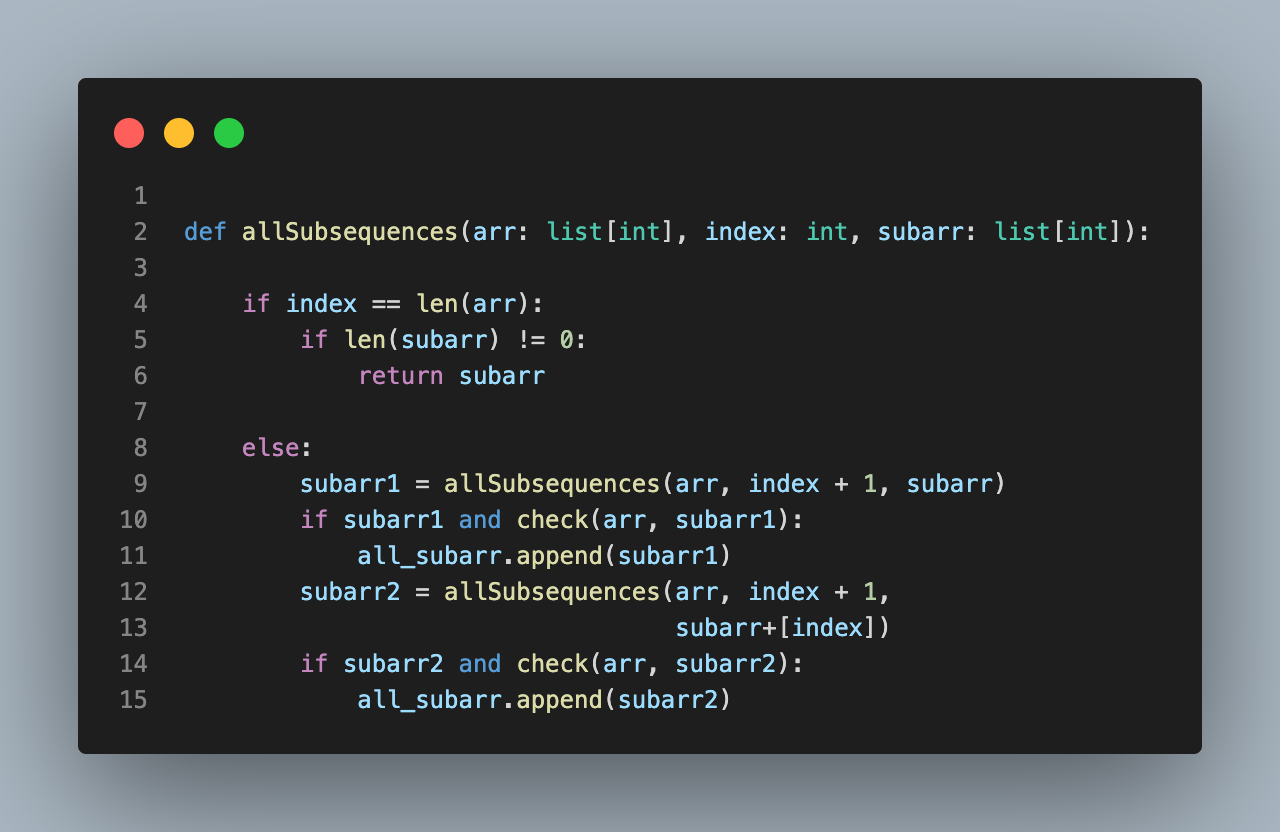
\includegraphics[width=0.5\textwidth]{all_subsequence.png}
        \centering
        \caption{Algoritmo para encontrar todas las subsecuencias}
    \end{figure}

 \begin{figure}[htb]
        \centering
        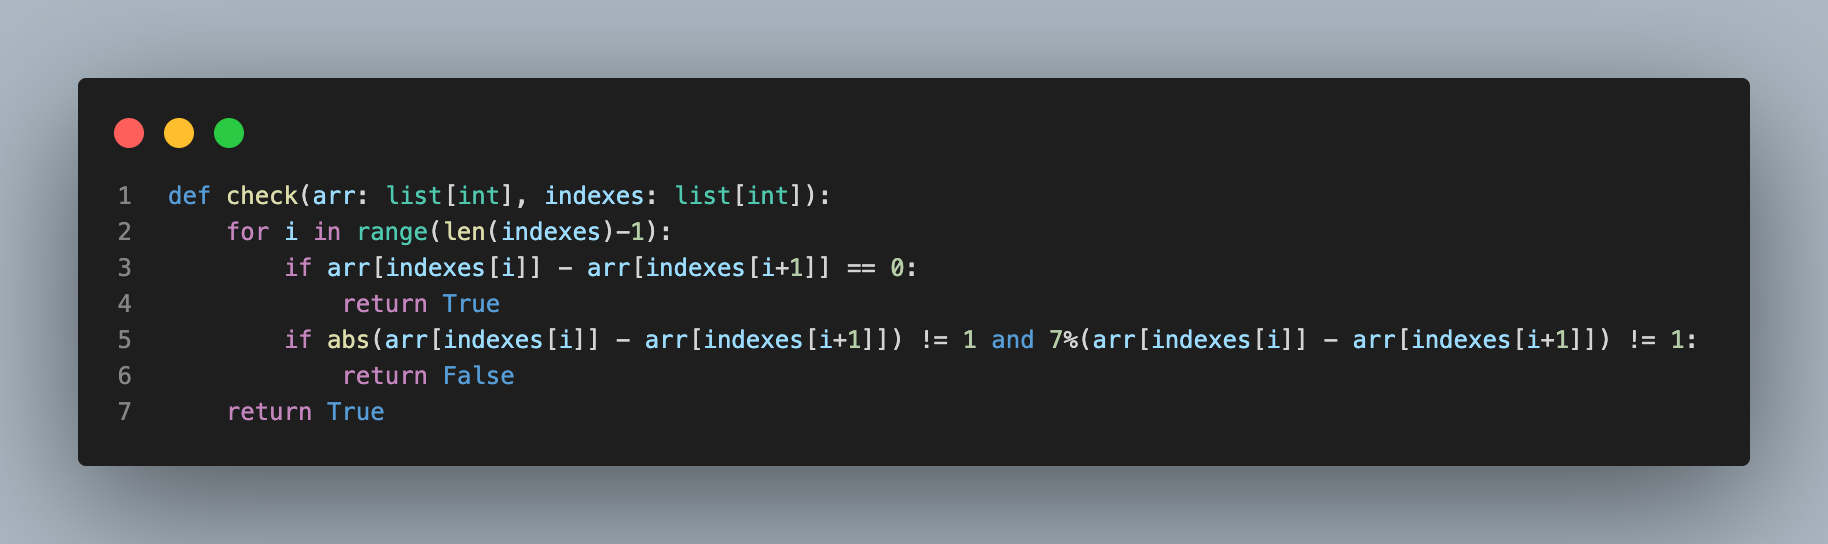
\includegraphics[width=0.5\textwidth]{check.png}
        \centering
        \caption{Algoritmo para chequear las condiciones del problema}
    \end{figure}

De cada subsecuencia guardamos sus índices y los guardamos la subsecuencia de los índices en una lista.
Una vez que tenemos esto pasamos a buscar todas la formas de obtener 4 melod\'ias sin que existan notas que se solapen, quedándonos con las 4 melod\'ias tal que la suma de sus longitudes sea la mayor(\textbf{Fig 3}).

 \begin{figure}[htb]
        \centering
        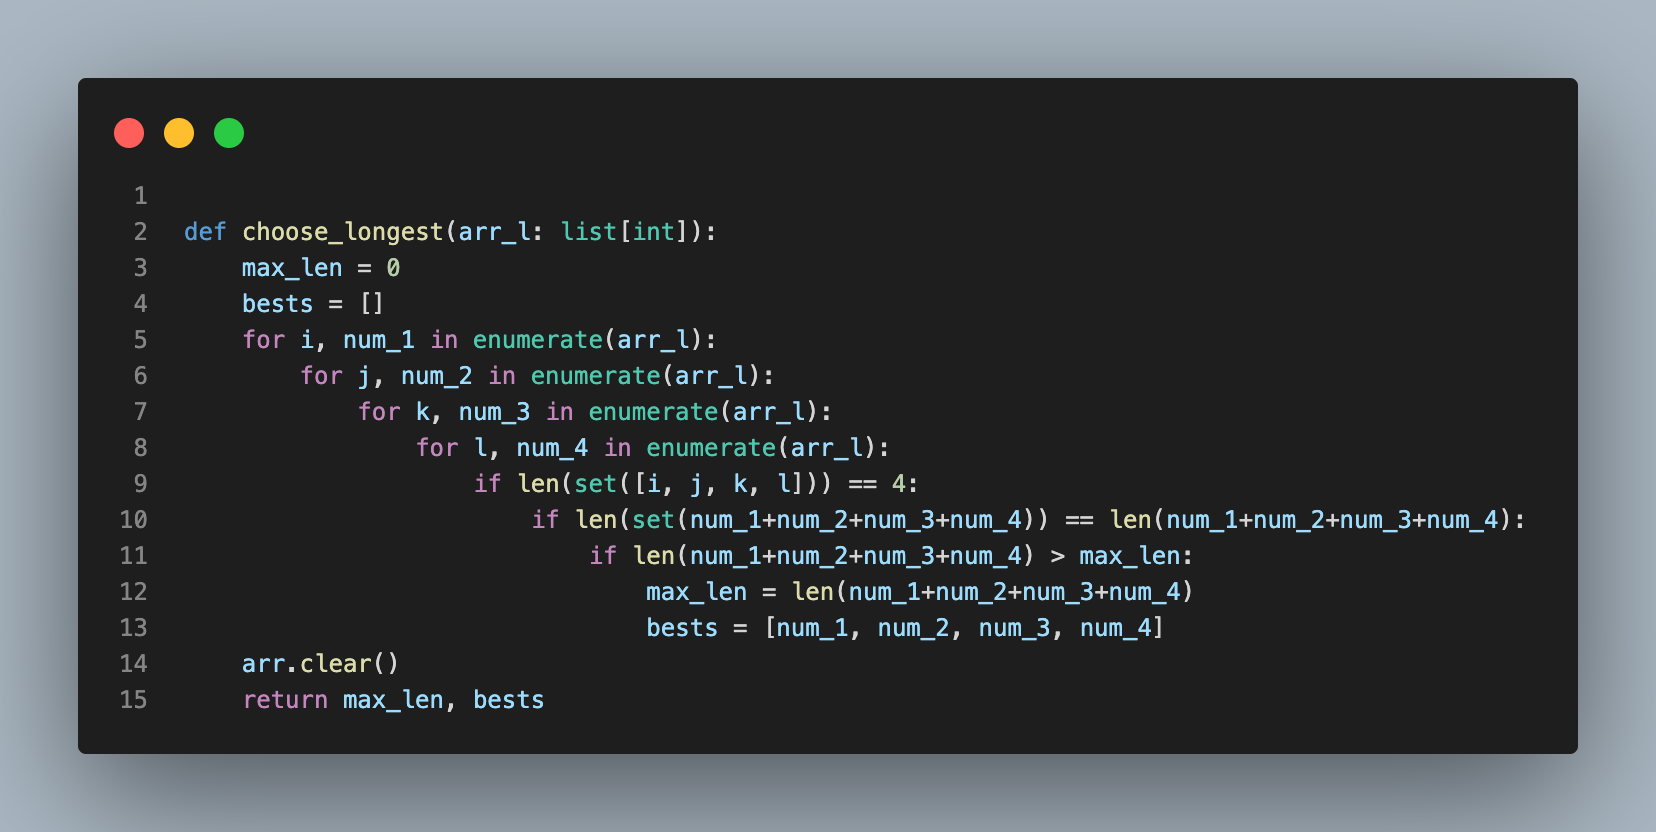
\includegraphics[width=0.5\textwidth]{choose_longest.png}
        \centering
        \caption{Algoritmo para obtener la melod\'ia que maximice el total de notas utilizadas}
    \end{figure}

\section*{An\'alisis de la complejidad temporal}
Encontrar toda las subsequencias de una lista de tama\~no n es $O(2^n)$ dada la implementaci\'on de la \textbf{Fig 1} ya que en cada llamada a la funci\'on, esta se llama así misma dos veces.\\
Encontrar las 4 melod\'ias que maximicen las notas utilizadas es en el peor de los casos $O(n^4)$ dada la implementaci\'on mostrada en la \textbf{Fig 3}\\

Por tanto con este primer acercamiento somos capaces de resolver el problema con costo computacional $O(n^4)$
\subsection{Peque\~na optimizaci\'on }
Una manera mas óptima de obtener las subsecuencias seria construyendo un grafo $G = (V,E)$ de la siguiente manera:
\begin{itemize}
    \item $\forall i \in V$ tal que $i<j ~ \exists(i,j) ~j \in V$ 
    \item A\~nadir un nodo $s$ y $\forall i\in V ~\exists(s,i)$
    \item A\~nadir un nodo $e$ y $\forall i\in V ~\exists(i,e)$
\end{itemize}
Una vez que tenemos esta estructura realizamos DFS desde $s$ hasta $e$ y cada vez que el algoritmo llegue hasta el final guardamos la camino por el que ha llegado quitando el nodo inicial y final. La complejidad temporal de este algoritmo ser\'ia el costo de DFS es decir $O(V + E)$ donde $V = n$ y $E$ es a lo sumo $n^2$ es decir la complejidad es $O(n^2)$ 
$

\section{Buscando una soluci\'on mas óptima }
Veamos cual es nuestro objetivo en este problema, es encontrar 4 subsecuencias que cumplan \textbf{(1)} y \textbf{(2)}  y además que no se solapen en una lista de forma tal que de forma tal que la suma de la longitud de estas subsecuencias sean lo mayor posible.\\
Para la resoluci\'on de este problemas transitamos por una modelaci\'in que nos aseguraba que las subsecuencias no se solaparan pero no aseguraba que tomáramos 4 subsecuencia tal que la suma de sus tama\~nos sea máxima.


\subsection*{Primera modelaci\'on}
Una vez que tenemos todas las subsequencias v\'alidas para nuestro problema dado una lista de enteros, creamos un grafo $G = (V,E)$ de la siguiente manera :\\
Cada nodo $v \in V $ va representar una subsecuencia v\'alida de la cadena.\\
Guardaremos todas las subsecuencias v\'alidas $S$ donde $S$ es una lista de lista de subsecuencias.
\begin{itemize}
    \item  $\forall i \in V$ tal que $i<j ~ \exists(i,j) ~j \in V$ 
    \item $\forall s_i,s_j \in S$ si $s_i$ y $s_j$ se solapan entonces $\exists v_k \in V$ tal que $\exists (v_k,s_i)~y~(v_k,s_j)$
    \item A\~nadir un nodo $s$ y $\forall v_k\in V $ tal que $v_k$ cumple lo planteado en el punto anterior entonces $\exists(s,v_k)$
    \item A\~nadir un nodo $e$ y $\forral i\in V ~\exists(i,e)$
    \item $\forall e \in E$ c(e) = 1
\end{itemize}
Una vez que tenemos esta estructura\textbf{Fig 4} podemos aplicar cualquiera de los algoritmos de flujo conocidos ya sea Ford–Fulkerson o Edmonds–Karp.\\
\begin{figure}[htb]
        \centering
        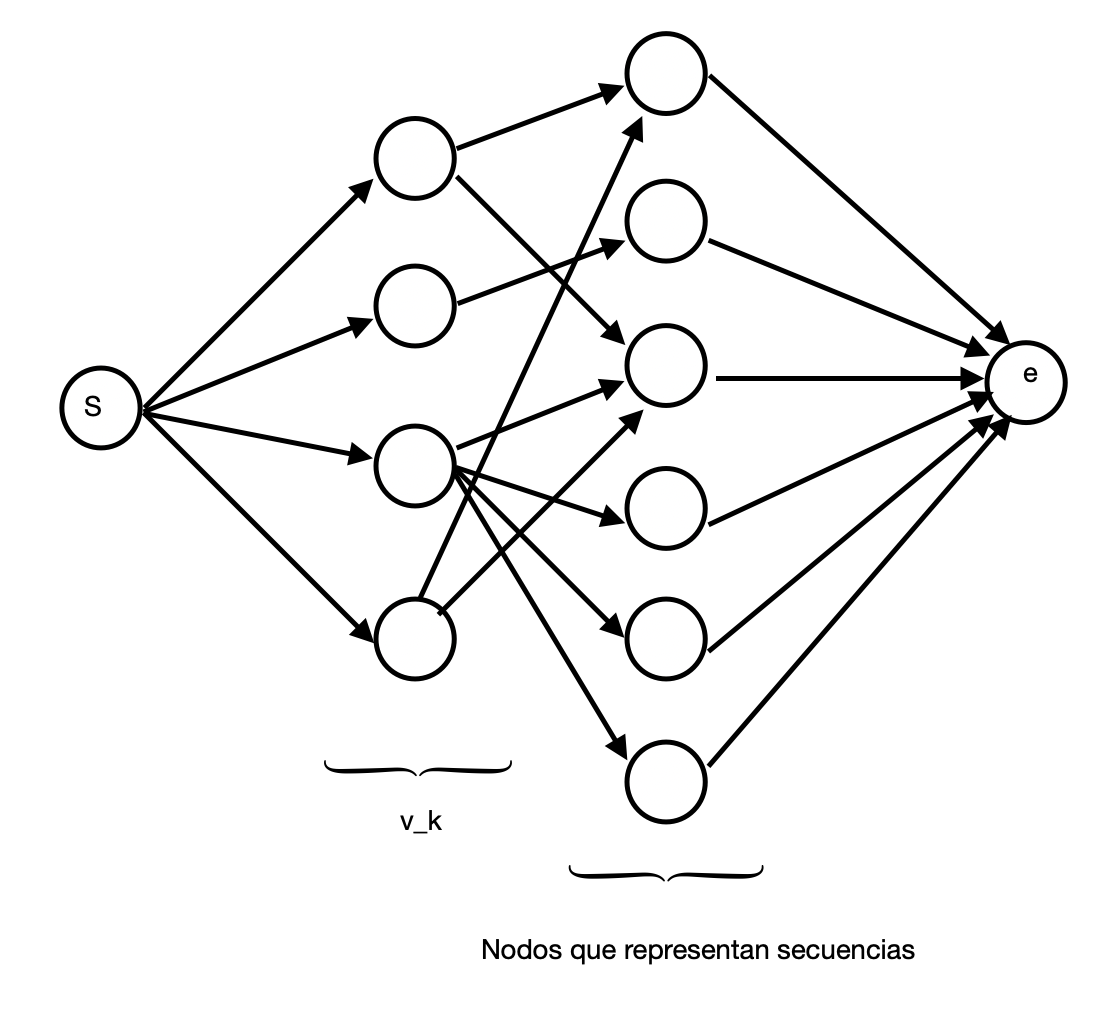
\includegraphics[width=0.8\textwidth]{Screenshot 2023-05-06 at 12.57.09 AM.png}
        \centering
        \caption{Estructura del grafo para la primera modelaci\'on}
    \end{figure}
Notemos que al tener los nodos $v_k$ y las aristas con capacidad 1
nos aseguramos de no tomar aristas solapadas, sin embargo esta modelaci\'on no nos da una soluci\'on factible a nuestro problema, ya que con esto no nos basta para asegurar que estamos maximizando la suma del tama\~no de las subsecuencias tomadas.\\
\textbf{¿ Qu\'e necesitamos ?}\\
Necesitamos encontrar alguna manera de tener en cuenta el tama\~no de la secuencia, para esto podr\'iamos intentar hacer el siguiente cambio en la capacidad de las aristas:
\begin{itemize}
    \item $\forall v_k,v_i \in V~si \exists~entonces(v_k,v_i) ~c(v_k,v_i) = 1$
    \item $\forall v_i \in V ~si \exists(v_i,e)~ entonces~c(v_i,e) = $ tama\~no de la subsecuencia que representa $v_i$
\end{itemize}
Note que al realizar flujo m\'aximo sobre este nuevo grafo estar\'iamos obteniendo el mismo resultado que en el grafo anterior ya que la m\'axima cantidad de flujo que puede salir de s es 4.\\
En conclusi\'on esta modelaci\'on no nos da resultados satifactorios, pero nos provee de una "buena idea" o "buena pregunta" ¿ podemos encontrar un algoritmo que combine flujo con costo?  
La respuesta es si, su nombre es flujo máximo-costo mínimo. \\
\section{Flujo m\'aximo costo m\'inimo}
Antes de adentrarnos en las premisas necesarias para poder correr este algoritmo y su funcionamientos, es necesario dominar algunos conceptos.
\begin{itemize}
    \item \textbf{Red de flujo :} Una red de flujo es un grafo dirigido, donde cada arista (u,v) tiene una capacidad no negativa $c(u,v) \geq 0$. Además se requiere que si $(u,v) \in E $ entonces $(v,u) \notin E$. Si $(u,v) \notin E $ entonces por conveniencia definimos que $c(u,v) = 0$ y además decimos que no existen lazos. Cada red de flujo contiene dos vértices distinguidos $s$ que es la fuente y $t$ que es el receptor. Es decir por cada vertice $v\in V$ existe un camino de s a v y de v a t\cite{1}.\\
    \item \textbf{Flujo :}\cite{2} Sea $G = (V,E)$ una red de flujo con una funci\'on de capacidad c. Sea s el vértice fuente y t el vértice receptor. Un \textbf{flujo} en G es una funci\'on de evaluaci\'on ~~ \textit{f} : VxV $\rightarrow$ R que satisface las siguientes propiedades:
    \begin{itemize}
        \item Limitación de capacidad: $\forall u,v $ se cumple que  $0 \leq f(u,v) \leq c(u,v)$
        \item Ley de conservación de flujo: $\forall v \in V -\{s,t\}$ se cumple que $\sum_{v\in V}f(v,u) = \sum_{v\in V}f(u,v)$
    \end{itemize}
    \item \textbf{Valor del flujo :}\cite{2} El valor del flujo ($|F|$) es definido como:\\
    ~~~~~$F = \sum_{v\in V}f(s,v) - \sum_{v\in V}f(v,s)$
    \item \textbf{Red de flujo residual :}\cite{3} Dada una red de flujo $G=(V,E)$ y un flujo \textit{f}, la red residual de $G$ inducida por \textit{f} es $G_f=(V,E_f)$, donde $E_f = \{(u,v)\in V$x$V :c_f(u,v) > 0\}$\\
    Una red residual $G_f$ consiste cuyas capacidades representan como puede cambiar el flujo en G.
    \item \textbf{Costo de un flujo:} Dada una red de flujo $G = (V,E)$ y una función de costo \textit{g} : E$\rightarrow$ R, el costo de un flujo \textit{f} en G es:\\
    $cost(f) = \sum_{e\in E}f(e)*c(e)$
\end{itemize}
Este algoritmo trabaja sobre una red de flujo con costo en las aristas; formalicemos esto.\\
Dada una red de flujo G, \textit{f} un flujo sobre G y \textit{g} una función de costo sobre G, definiremos el grafo de flujo máximo - costo mínimo como $G_{f,c} = (V,E_{f,c},c,cost)$ donde para toda $e \in E$ se le asocia la tupla $[c,cost]$, donde c es la capacidad y cost el costo.\\
Dado una red de flujo máximo - costo mínimo como $G_{f,c} = (V,E_{f,c},c,cost)$ y un flujo $f$ definimos la red residual de $G_{f,c}$ como $G_r = (V,E_r)$, donde $\forall e = (u,v) \in E$  si $f(e) < c(e)$ entonces $G_r$ tiene una arista $e = (u,v)$ con capacidad $c_r = c(e) - f(e)$ y costo $cost_r(e) = cost(e)$ y si $0 < f(e)$ entonces $G_r$ tiene una arista $e^{'} = (v,u)$ con capacidad $c_r(e^{'}) = f(e)$ y costo $cost(e^{'}) = -cost(e)$\\
Notemos que el hecho de que las aristas reversas tienen costo con signo opuesto a las originales. Poner flujo en $e^'$ representa remover flujo desde $e$ y si hacemos esto esto queremos de vuelta el costo de haber puesto flujo por la arista $e$\\

\textbf{Teorema 5:} Dada una red de flujo $G = (V,E)$ y un flujo f. El flujo f puede ser descompuesto en caminos y ciclos, existen un conjunto finito A, de P de caminos de s a t y y ciclos C de s a t. Cada camino P y cada ciclo C tiene un peso positivo llamémosle w(P) y w(C) respectivamente, tal que:
$$f(e) = \sum_{p\in A,e\in P}w(P) + \sum_{c\in A,e\in C} w(c)$$
Es decir, el flujo en cada arista es el peso total de todos los caminos y ciclos que pasan por ella.\\

\textbf{Nota1}: Sea $G=((V,E),c,a)$ una red de flujo sin ciclos negativos. Sea f un flujo en G obtenido tomando algún camino de costo mínimo P desde s a t y poniendo $\gamma$ flujo en cada arista de P. Entonces $G_r$ no tiene ciclos negativos.\\
Demostración:\\
Supongamos que después de unos pasos aumentativos iniciales tenemos flujo x y $G_r$ no contiene ciclos negativos. Denotemos el próximo camino de costo mínimo encontrado como P. Supongamos que después de aumentar el flujo por sobre el camino P aparece un ciclo W de costo negativo en la red residual, 
esto significa que había una arista (i,j) en P donde el reverso (j,i) cerro el ciclo W después del aumento. Entonces podríamos coger otro camino de s a t tal q s vaya a i, luego de i a j a través de las aristas de W y de j a t, este camino tendría menor costo que P por lo q ser\'ia una contradicción.\\

\textbf{Nota2} Sea $G=((V,E),c,a)$ una red de flujo y f un flujo, $G_r$ no tiene ciclos de costo negativo si y solo si f tiene costo mínimo entre todos los flujos con $|f|$. \cite{4}\\


El algoritmo de flujo maximo - costo mínimo se auxilia de algoritmos como Dinitz, Bellman-Ford\cite{5} y Dijkstra\cite{6}.\\

\textbf{Algoritmo de Dinitz}
Es un algoritmo para calcular el flujo máximo en una red de flujo, tiene complejidad $O(V^2E)$\cite{7}\cite{4}


Sea $G=((V,E),c,a)$ una red de flujo sin ciclos negativos, se denota $dist(u,v)$ el costo del camino de costo mínimo desde u a v. El subgrafo de caminos de costo mínimos de G contiene todas las aristas e desde u hasta v tal que:
$$dist(s,u) + cost(u,v) = dist(s,v)$$

Sea $G=((V,E),c,a)$ una red de flujos sin ciclos negativos, sea S el subgrafo de caminos de costo mínimo en G y f un flujo en S entonces $G_r$ no tiene ciclos negativos.\\
Demostración: \\
Descomponemos f en caminos y ciclos, empezamos añadiendo los caminos de uno en uno. Supongamos que algunos caminos ya fueron añadidos. Vamos a añadir el camino $p_i$ como la longitud del camino de costo nunca disminuye entonces todavía ser\'a un camino de costo mínimo. Si la red residual no tenia ciclos negativos antes de añadir $p_i$ tampoco los tendrá después de añadirlo(\textbf{Nota1}).\\
Los ciclos en S deben tener costo cero por lo tanto esto pueden ser añadidos sin cambiar el valor o el costo del flujo, si el flujo era mínimo antes, también lo sera después, al final del proceso la red residual que obtenemos es exactamente $G_r$ y no tiene ciclos negativos.\\

Trabajar con pesos negativos es importante por lo que necesitamos desarrollar una manera efectiva de encontrar subgrafos de costo mínimo que implica encontrar caminos de costo mínimo. Con aristas de costo negativo Dijkstra no funciona correctamente, por lo que el mejor método clásico para encontrar caminos de costo mínimo desde s ser\'ia Bellman-Ford con costo cuadrático, sin embargo, hay una mejor manera de encontrar los caminos de costo mínimo que usar Bellman-Ford cada vez.\\

Sea G un grafo dirigido con costos en las aristas $a: E \rightarrow R$ y $p: V \rightarrow R$ una función. Redefinimos el costo de las aristas e que va de (u,v) como :
$$a_p(e) = p(u) +a(e) - p(v)$$

Luego dado un grafo dirigido G, el costo de las aristas $a: E\rightarrow R$ y un mapeo $p: V\rightarrow R$ para cualquiera dos vértices u,v los caminos de costo mínimo de u a v con respecto a la funciona a son exactamente los caminos de costo mínimo de u a v con respecto a $a_p$.\\
Esto significa que si queremos encontrar caminos de costo mínimo podríamos tomar un p y reemplazar el costo de las aristas de esta manera, si pudiéramos escoger p tal que el costo de todas las aristas se convirtieran en no negativos, podríamos utilizar Dijkstra para encontrar caminos de costo mínimo.\\
Dado G un grafo dirigido con costos en las aristas $a: E \rightarrow R$ y $p: V \rightarrow R$ se la llama potencial si $a_p$ en E es mayor o igual que cero para todas las aristas\\

Dado G un grafo dirigido con costos en las aristas $a: E \rightarrow R$ tal que no hay ciclos negativos, sea s un vértice tal que para todo vértice alcanzable desde s, si se define p(v) como la longitud del camino de costo mínimo desde s hasta v, entonces p es un potencial.\\
Demostración:\\
Sea una arista desde u hasta v. Tenemos que demostrar que:
$$p(u) + a(e) \geq p(v)$$
lo cual es verdad porque sino podríamos obtener un camino mas corto desde s a v pasando por u y e.

    \begin{figure}[htb]
        \centering
        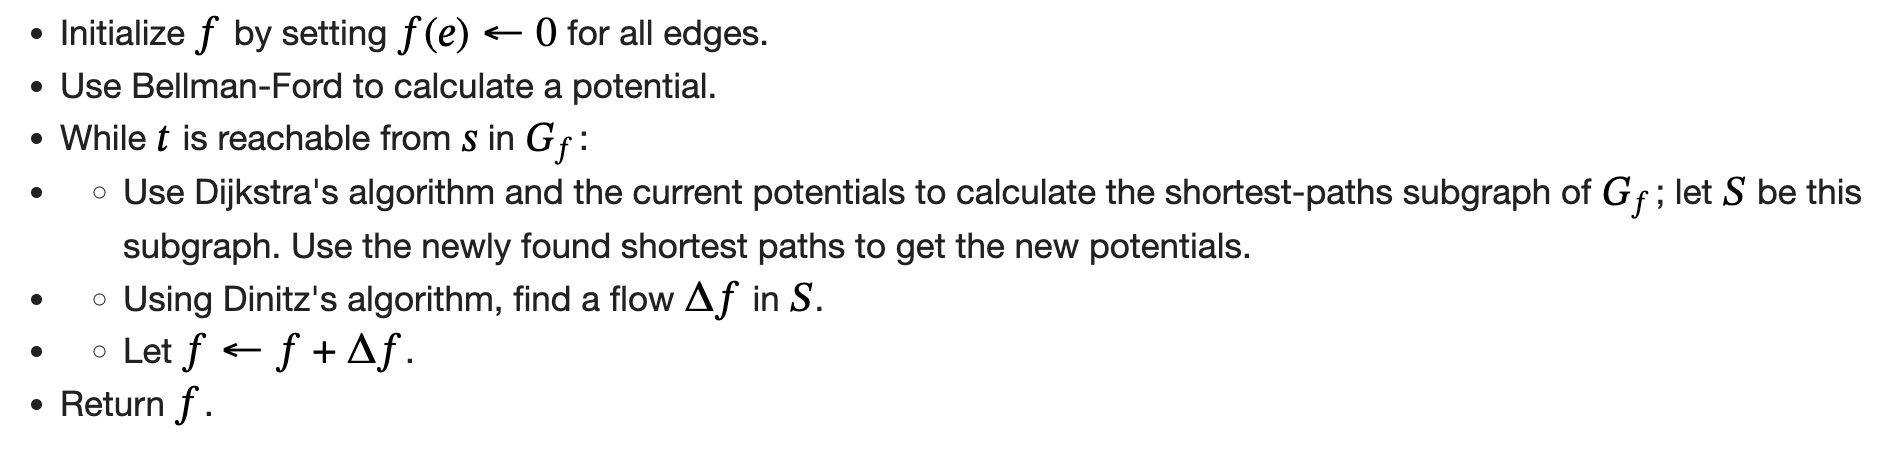
\includegraphics[width=1.3\textwidth]{algorithm_2.png}
        \centering
        \caption{Algoritmo de flujo máximo costo mínimo }
    \end{figure}
\\

Debido a las \textbf{Nota1} y \textbf{Nota2}  podemos afirmar que el flujo f siempre sera el costo mínimo sin importar el valor en el que este. Y con esto queda demostrada la correctitud del algoritmo.\\

\subsection*{Análisis de complejidad:}
\begin{enumerate}
    \item $O(E)$
    \item $O(V^2 + VE)$
    \item $O(ELogV)$
    \item $O(V^2E)$
    \item $O(E)$
\end{enumerate}

Como el ciclo de la l\'inea 3 se ejecuta $O(V)$ veces, la complejidad total del algoritmo es $O(V^3E)$

\subsection{Adaptación de nuestro problema a uno de flujo máximo-costo mínimo}
Llamaremos a \textbf{l} a la lista input del problema 
Para nuestro problema construimos un grafo $G=(V,E)$ donde :\\
\begin{itemize}
    \item $V = \{ v : v\in l\}$.
    \item  $E = \{(u,v): u,v \in V y~ pos(u) < pos(v) y \}$.
    \item Se añaden a V los vértices s, que representa la fuente, t que representa el destino, además de los vértices 
    \item Al añadir el vértice s se añaden a E las siguientes aristas: $\forall v \in V$ se ande la arista (s,v).
    \item Se añaden además los siguientes vértices a V $t_1,t_2,t_3,t_4$ que van a representar las melodías 1,2,3 y 4 respectivamente.
    \item Al añadir los vértices $t_1,t_2,t_3,t_4$ se añaden a E las siguientes aristas $(v,t_1),(v,t_2),(v,t_3),(v,t_4) \forall v \in V$.
    \item Se añaden a E las siguientes aristas $(t_1,s),(t_2,s),(t_3,s),(t_4,s)$
    \item Por cada vértice en v se crea un duplicado $v^'$ que se añade a V y además se crea la arista $(v,v^{'})$, y se actualiza E de la siguiente manera: $\forall e = (v,x) in E $ eliminamos la arista e de E y en su lugar añadimos la arista $e^{'} = (v^{'},x)$.
    
    
\end{itemize}
\begin{thebibliography}{99}
\bibitem{1} thomas-h-cormen-introduction-to-algorithms-4th-edition parte VI cap 24 page 671
 \bibitem{2} thomas-h-cormen-introduction-to-algorithms-4th-edition parte VI cap 24 page 672
 \bibitem{3} thomas-h-cormen-introduction-to-algorithms-4th-edition parte VI cap 24 page 677
\bibitem{4} Ravindra K. Ahuja, Thomas L. Magnanti, and James B. Orlin. Network Flows: Theory, Algorithms, and Applications.
\bibitem{5} thomas-h-cormen-introduction-to-algorithms-4th-edition parte VI cap 22 page 612
\bibitem{6} thomas-h-cormen-introduction-to-algorithms-4th-edition parte VI cap 22 page 620
\bibitem{7} https://es.wikipedia.org/wiki/Algoritmo-de-Dinic
\end{thebibliography}

\end{document}



